\documentclass[a4paper,14pt]{extarticle}
\usepackage{../../tex-shared/report-layout}

\renewcommand{\mylabnumber}{2}
\renewcommand{\mylabtitle}{Исследование
возможностей программирования
на стороне клиента. Основы языка JavaScript}
\renewcommand{\mysubject}{Веб-технологии}
\renewcommand{\mylecturer}{Дрозин А.Ю.}

\begin{document}
\begin{titlepage}
    
    \thispagestyle{empty}
    
    \begin{center}
        
        Министерство науки и Высшего образования Российской Федерации \\
        Севастопольский государственный университет \\
        Кафедра ИС
        
        \vfill

        Отчет \\
        по лабораторной работе №\mylabnumber \\
        \enquote{\mylabtitle} \\
        по дисциплине \\
        \enquote{\MakeTextUppercase{\mysubject}}

    \end{center}

    \vspace{1cm}

    \noindent\hspace{7.5cm} Выполнил студент группы ИС/б-17-2-о \\
    \null\hspace{7.5cm} Горбенко К. Н. \\
    \null\hspace{7.5cm} Проверил \\
    \null\hspace{7.5cm} \mylecturer

    \vfill

    \begin{center}
        Севастополь \\
        \the\year{}
    \end{center}

\end{titlepage}

\section{Цель работы}
Изучить основы языка JavaScript и объектной модели браузера,
приобрести практические навыки проверки HTML-форм с использованием
JavaScript.

\section{Задание на работу}
\begin{enumerate}
    \item Модифицировать страницу «Фотоальбом» (использовать
          HTMLстраницы, разработанные при выполнении предыдущей
          лабораторной работы), реализовав вывод таблицы,
          содержащей фото, с использованием операторов циклов.
          Значения имен файлов фото и подписей к фото
          предварительно разместить в массивах fotos и titles.
    \item Модифицировать страницу «Мои интересы», реализовав вывод
          списков с использованием JavaScript-функции с переменным
          числом аргументов.
    \item Добавить на страницах «Контакт» и «Тест по дисциплине «…»»
          функции проверки заполненности форм. В случае если
          какое-либо из полей формы осталось незаполненным при нажатии
          на кнопку отправить, вывести сообщение об ошибке и
          установить фокус на незаполненный элемент.
    \item Добавить на странице «Контакт» текстовое поле «Телефон».
          И для полей «Фамилия Имя Отчество» и «Телефон» добавить
          функции специфической проверки значений. В случае если
          какое-либо из полей формы заполнено не верно, при нажатии
          на кнопку отправить, вывести сообщение об ошибке и установить
          фокус на неверно заполненный элемент. Формат правильных
          значений полей:
          
          \begin{itemize}
              \item Фамилия Имя Отчество – введено три слова,
                    разделенные одним пробелом.
              \item Телефон – строка может состоять только из цифр;
                    начинаться только с последовательности «+7» или «+3»;
                    не содержит пробелов; количество цифр в строке от
                    9 до 11.
          \end{itemize}
    \item Добавить на странице «Тест по дисциплине «…»» функции
          специфической проверки значений полей в соответствии
          с вариантом задания. В случае не выполнения условия
          сформировать сообщение об ошибке и установить фокус
          на неверно заполненный элемент ввода.
    \item Необходимо выполнить проверку разработанных JavaScript
          файлов с использованием сервиса jshint.
\end{enumerate}
\textbf{Вариант № 3}: 3 вопрос, количество слов в ответе не более 30.

\section{Ход работы}
\subsection{Страница \enquote{Фотоальбом}}
Для выведения фотографий средствами языка JavaScript была написана\
следующая программа:
\begin{lstlisting}
window.onload = () => {
    let photoWrapper = document.getElementsByClassName('photo-wrapper').item(0);
    photos.forEach(photo => {
        let img = document.createElement('img');
        img.setAttribute('src', photo);
        img.setAttribute('alt', 'photoalbum photo');
        photoWrapper.appendChild(img);
    });
};
const photos = [
    'picachu.jpg',
    'images.jpeg',
    'lion-king.jpg',
    'road.jpeg',
    'car.png',
    'bridge.jpg',
    'green.jpeg',
    'statue.jpg',
    'cock.jpg',
    'city.jpg',
    'fire.jpg',
    'rose.jpeg',
    'photo.jpg',
    'castrle.jpg',
    'shimpanze.jpg',
].map(image => image = `../images/${image}`);
\end{lstlisting}

В данной программе пути к фото хранятся в массиве \code{photos}.
При загрузке страницы происходит вызов функции, которая в цикле
добавляет фото в документ.

\subsection{Страница \enquote{Мои интересы}}
На данной странице функция \code{loadInterests} c переменным
числом аргументов используется для выведения списков:
\begin{lstlisting}
window.onload = () => {
    let links = document.getElementsByClassName('contents');
    const interestsKeys = Object.keys(interests);
    loadInterests(interestsKeys[0], interestsKeys[1], interestsKeys[2], interestsKeys[3]);
};

const loadInterests = (...interestsIds) => {
    const interestsList = document.getElementById('interests');
    interestsIds.forEach(interestId => {
        const content = interests[interestId];
        let interestWrapper = document.createElement('div');
        interestWrapper.setAttribute('id', interestId);
        interestWrapper.appendChild(createElement('h2', content.header));
        interestWrapper.appendChild(createElement('p', content.values[0]));
        interestWrapper.appendChild(createElement('p', content.values[1]));
        interestsList.appendChild(interestWrapper);
    });
};

const createElement = (tagName, content) => {
    let element = document.createElement(tagName);
    element.innerHTML = content;
    return element;
};

const interestContent = `Lorem ipsum dolor sit amet, consecteturadipiscing elit. Sed gravida
    dolor et ultricies placerat. Pellentesque in lectus at augue rutrum 
    volutpat vel sed tellus. Donec feugiat ac nibh et pharetra. Curabitur 
    fringilla lacinia nisl tempus mollis. Nam semper augue et ante ornare
    semper. Etiam nunc velit, pharetra eget fermentum tincidunt, lacinia 
    vitae sapien. Etiam quis elit tincidunt, consequat urna eget, vulputate
    libero. Donec dignissim ornare porttitor. Donec id augue turpis. Morbi massa 
    sem, dapibus at semper in, mollis a sem. Ut eu lacus ut leo aliquam laoreet. 
    Integer sed ex vel erat dictum finibus sit amet id mi. Duis lorem neque, 
    faucibus ut laoreet eu, sodales in orci. Nam mattis mauris sit amet lectus
    condimentum, in maximus massa ultrices. Fusce pharetra accumsan dui sed bibendum.`;

const interests = {
    'Hobbies': {
        header: 'My hobbies',
        values: [
            'My hobbies are supposed to be here',
            interestContent
        ]
    },
    'Books': {
        header: 'My books',
        values: [
            'My books are supposed to be here',
            interestContent
        ]
    },
    'Music': {
        header: 'My music',
        values: [
            'My music is supposed to be here',
            interestContent
        ]
    },
    'Films': {
        header: 'My films',
        values: [
            'My films are supposed to be here',
            interestContent
        ]
    }
};
\end{lstlisting}

Списки хранятся в объекте \code{interests}, выводятся с помощью
функции с одним rest-параметром, в которую передаются элементы массива.

\subsection{Страницы \enquote{Контакт} и \enquote{Тест}}
На данных страницах добавлено поле \enquote{Номер телефона}. На все поля
добавлена валидация с выводом сообщений и установкой фокуса на
неправильно введенных полях. Тексты программ представлены далее.
Текст файла \code{contact.js}:
\begin{lstlisting}
class FieldFilledValidator {
    constructor() {
        this.errorMessage = 'This field should be filled';
        this.validate = (value) => {
            return value !== '';
        };
    }
}
class PhoneNumberValidator {
    constructor() {
        this.errorMessage = 'Entered number is in incorrect format';
        this.validate = (value) => {
            const pattern = /^[+][7|3]\d{8,10}$/g;
            return pattern.test(value);
        };
    }
}
class NameValidator {
    constructor() {
        this.errorMessage = 'Enter three space-separated words';
        this.validate = (value) => {
            const pattern = /[A-Za-z]+ [A-Za-z]+ [A-Za-z]+/;
            return pattern.test(value);
        };
    }
}
class FormComponent {
    constructor(componentId, validators) {
        this.validate = () => {
            this.validators.forEach(validator => {
                const message = validator.errorMessage;
                if (validator.validate(this.value)) {
                    this.errorMessages.splice(this.errorMessages.indexOf(message), 1);
                }
                else {
                    if (!this.errorMessages.includes(message)) {
                        this.errorMessages.push(message);
                    }
                }
            });
        };
        this.componentId = componentId;
        this.validators = validators;
        this.errorMessages = [];
    }
    ;
}
const fields = [
    new FormComponent('full-name-input', [
        new NameValidator(),
    ]),
    new FormComponent('email-input', [
        new FieldFilledValidator(),
    ]),
    new FormComponent('phone-input', [
        new PhoneNumberValidator(),
    ]),
    new FormComponent('message-input', [
        new FieldFilledValidator(),
    ]),
];
window.onload = () => {
    const form = document.forms.item(0);
    form.addEventListener('submit', validateForm);
    fields.forEach(field => {
        const fieldElement = document.getElementById(field.componentId);
        fieldElement.addEventListener('change', () => validateField(field));
    });
};
const validateField = (field) => {
    const errorsMessages = document.getElementById(`${field.componentId}-errors`);
    if (errorsMessages !== null) {
        errorsMessages.remove();
    }
    field.value = document.getElementById(field.componentId).value;
    field.validate();
    if (field.errorMessages.length > 0) {
        showMessages(field);
    }
};
const validateForm = () => {
    let firstError;
    fields.forEach(field => {
        validateField(field);
        if (!firstError && field.errorMessages.length > 0) {
            firstError = field;
        }
    });
    if (firstError) {
        document.getElementById(firstError.componentId).focus();
    }
    if (fields.some(field => field.errorMessages.length > 0)) {
        event.preventDefault();
    }
};
const showMessages = (field) => {
    const targetElement = document.getElementById(field.componentId);
    const parentElement = targetElement.parentElement;
    let contentWrapper = document.createElement('div');
    contentWrapper.setAttribute('id', `${field.componentId}-errors`);
    contentWrapper.setAttribute('class', 'error-messages');
    field.errorMessages.forEach(message => {
        let messageListItem = document.createElement('li');
        messageListItem.innerHTML = message;
        contentWrapper.appendChild(messageListItem);
    });
    parentElement.insertBefore(contentWrapper, targetElement);
};
\end{lstlisting}

Текст файла \code{test.js}:
\begin{lstlisting}
class FieldFilledValidator {
    constructor() {
        this.errorMessage = 'This field should be filled';
        this.validate = (value) => {
            return value !== '';
        };
    }
}
class PhoneNumberValidator {
    constructor() {
        this.errorMessage = 'Entered number is in incorrect format';
        this.validate = (value) => {
            const pattern = /^[+][7|3]\d{8,10}$/g;
            return pattern.test(value);
        };
    }
}
class NameValidator {
    constructor() {
        this.errorMessage = 'Enter three space-separated words';
        this.validate = (value) => {
            const pattern = /[A-Za-z]+ [A-Za-z]+ [A-Za-z]+/;
            return pattern.test(value);
        };
    }
}
class FormComponent {
    constructor(componentId, validators) {
        this.validate = () => {
            this.validators.forEach(validator => {
                const message = validator.errorMessage;
                if (validator.validate(this.value)) {
                    this.errorMessages.splice(this.errorMessages.indexOf(message), 1);
                }
                else {
                    if (!this.errorMessages.includes(message)) {
                        this.errorMessages.push(message);
                    }
                }
            });
        };
        this.componentId = componentId;
        this.validators = validators;
        this.errorMessages = [];
    }
    ;
}
const fields = [
    new FormComponent('full-name-input', [
        new NameValidator(),
    ]),
    new FormComponent('email-input', [
        new FieldFilledValidator(),
    ]),
    new FormComponent('phone-input', [
        new PhoneNumberValidator(),
    ]),
    new FormComponent('message-input', [
        new FieldFilledValidator(),
    ]),
];
window.onload = () => {
    const form = document.forms.item(0);
    form.addEventListener('submit', validateForm);
    fields.forEach(field => {
        const fieldElement = document.getElementById(field.componentId);
        fieldElement.addEventListener('change', () => validateField(field));
    });
};
const validateField = (field) => {
    const errorsMessages = document.getElementById(`${field.componentId}-errors`);
    if (errorsMessages !== null) {
        errorsMessages.remove();
    }
    field.value = document.getElementById(field.componentId).value;
    field.validate();
    if (field.errorMessages.length > 0) {
        showMessages(field);
    }
};
const validateForm = () => {
    let firstError;
    fields.forEach(field => {
        validateField(field);
        if (!firstError && field.errorMessages.length > 0) {
            firstError = field;
        }
    });
    if (firstError) {
        document.getElementById(firstError.componentId).focus();
    }
    if (fields.some(field => field.errorMessages.length > 0)) {
        event.preventDefault();
    }
};
const showMessages = (field) => {
    const targetElement = document.getElementById(field.componentId);
    const parentElement = targetElement.parentElement;
    let contentWrapper = document.createElement('div');
    contentWrapper.setAttribute('id', `${field.componentId}-errors`);
    contentWrapper.setAttribute('class', 'error-messages');
    field.errorMessages.forEach(message => {
        let messageListItem = document.createElement('li');
        messageListItem.innerHTML = message;
        contentWrapper.appendChild(messageListItem);
    });
    parentElement.insertBefore(contentWrapper, targetElement);
};
\end{lstlisting}

На рисунках \ref{fig:contact-validation} - \ref{fig:form-validation}
изображены сообщения при нажатии на кнопку \enquote{Submit} при пустой форме.
\begin{figure}[H]
    \centering
    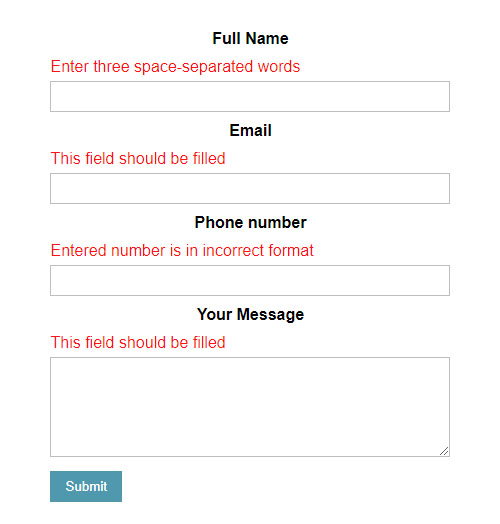
\includegraphics[width=.8\linewidth]{contact}
    \caption{Тексты сообщений при ошибке валидации на странице \enquote{Контакт}}
    \label{fig:contact-validation}
\end{figure}
\begin{figure}[H]
    \centering
    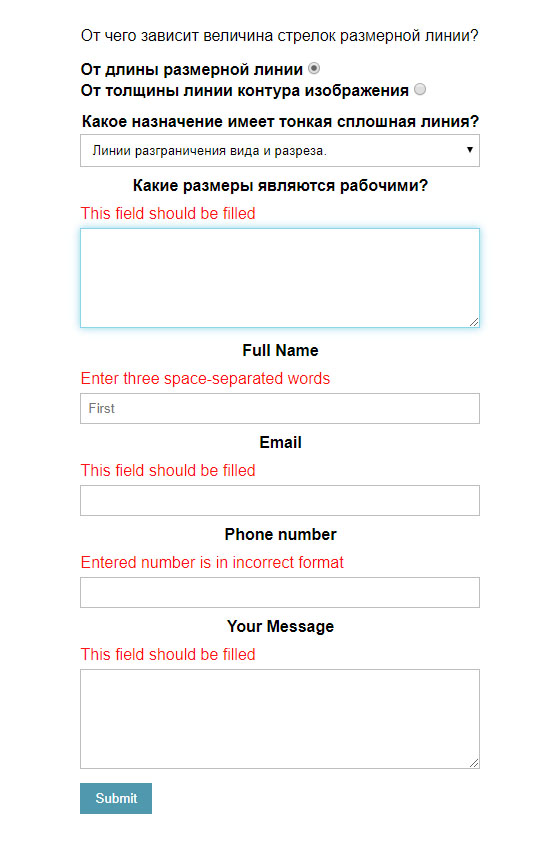
\includegraphics[width=.8\linewidth]{test}
    \caption{Тексты сообщений при ошибке валидации на странице \enquote{Тест}}
    \label{fig:form-validation}
\end{figure}

В данных программах создаются массивы элементов формы, в которых
к элементам привязываются классы валидации, содержащие саму
функцию валидации и сообщение об ошибке валидации. При изменении
любого из полей, на нем срабатывает функция валидации.

В формы добавлены поля \enquote{Номер телефона}. Поле \enquote{Имя} валидируется
как три слова, разделенные пробелом. Текстовое поле ответа на третий вопрос теста
требует менее 30 слов.

\section*{Выводы}
В ходе лабораторной работы были изучены способы получения и вставки элементов
\code{HTML}-документа. Для работы с \code{HTML} используется механизм
\code{DOM}, в котором каждый элемент документа представляет из себя объект
языка JavaScript.

Валидация проводилась с помощью функций, которые реагировали на событие
\enquote{change}. Привязка к полям документа осуществлялась по их id.
\end{document}